\newacronym{ai}{AI}{Artificial Intelligence}
\newacronym{ibv}{IBV}{industrielle Bildverarbeitung}
\newacronym{dl}{DL}{Deep Learning}
\newacronym{cnn}{CNNs}{Convolutional Neural Networks}
\newacronym{ann}{ANN}{Artificial Neural Networks}
\newacronym{bv}{BV}{Bildverarbeitung}
\newacronym{cv}{CV}{Computer Vision}
\newacronym{od}{OD}{Objektdetektion}



\chapter{Einleitung}\label{sec:exp_einleitung}

Die \gls{ibv} ist ein Teilgebiet des Maschinellen Sehens  auch \gls{cv} genannt. Die \gls{ibv} ermöglicht es Maschinen und Systemen, visuelle Informationen aus Produktionsprozessen und Produkten zu erfassen und auszwerten. Dadurch können Aufgaben wie Qualitätskontrolle, Inspektion, Positionierung und Vermessung durchgeführt werden. Im Vordergrund steht dabei immer, die Qualität transparent zu machen, um die Prozess- oder Produktqualität automatisch oder durch manuelles Eingreifen des Bedienpersonals zu verbessern. Durch den Einsatz von automatisierten Sichtprüfsystemen wird es möglich, mit geringen laufenden Kosten vollständige Prüfungen in der industriellen Fertigung durchzuführen. Im Vergleich zu stichprobenartigen Qualitätskontrollen werden so Reaktionszeiten verkürzt und damit Ausschusskosten reduziert.\citep{cognex_grundlagen_nodate} 

Die \gls{od} ist eine Technik der \gls{bv} dass die identifikation und erkennung von objekten in einem Bild oder Video ermöglicht. Die realisierung der Objektdetektion erfolgt mittels traditionelle \gls{bv}-algorithmen, Algorithmen mittels Maschinelles Leren und \gls{dl}-Algorithmen. Mit Hilfe von \gls{dl} können im Gegensatz zu herkömmlichen \gls{bv}-methoden auch komplexe und variierende Prüfaufgaben, die bisher der menschlichen Begutachtung vorbehalten waren, effizient und kostengünstig automatisiert werden.\cite{kaur_systematic_2024}

Der Einsatz von Deep Learning führt aber auch zu Veränderungen im Gesamtprozess. Neue Teilprozesse wie das Training von künstlichen neuronalen Netzen (von engl. \gls{ann}) sind bereits hinreichend wissenschaftlich untersucht. Ein Beispiel für die Anwendung von Objektdetektio mittels \gls{dl}-Modellen werden in der Industrie häufig zur Oberflächeninspektion von Produkten wie Metall, Gewebe und Stahl eingesetzt. Dazu gehört die Erkennung von Kratzern, Rissen und Verformungen auf der Oberfläche. \gls{cnn} sind eine der am häufigsten verwendeten Architekturen für diese Anwendung.\citep{saberironaghi_defect_2023}

In dieser Arbeit möchte ich die Entwicklung und Evaluierung einer \gls{dl}-Anwendung vorstellen, die bestimmte gelabelte Merkmale in Bildern aus der Industire automatisch erkennen kann. Dabei wird untersucht, wie mit Hilfe von \gls{cnn} und semantischer Segmentierung eine zuverlässige Erkennung bzw \gls{od} trotz Herausforderungen wie begrenzter Datenmenge und Bildrauschen möglich ist.

\section{Motivation}\label{expose_motivation}
Im Rahmen meines Praxissemesters bei der Gefasoft GmbH in Regensburg hatte ich die Gelegenheit, mich mit Projekten der \gls{ibv} zu befassen. Im Bildverarbeitungslabor wurde mir ein Einblick in die vielfältigen Prozesse einer Sichtprüfung im Bereich der \gls{ibv} gewährt.

In der industriellen Sichtprüfung wird überprüft, ob ein Prüfteil den spezifischen Vorgaben entspricht, beispielsweise hinsichtlich Abmessungen, Formen oder der Anwesenheit bestimmter Merkmale. Dieser Prozess umfasst mehrere aufeinanderfolgende Schritte, beginnend mit der Bildaufnahme und -vorverarbeitung, über die Identifikation relevanter Bildbereiche bis hin zur Analyse und Bewertung der Objekteigenschaften (Siehe Abbildung \ref{fig:vorgehensmodell} ) \cite[S. 15–16]{demant_industrielle_2011}.

\begin{figure}[h]
    \centering
    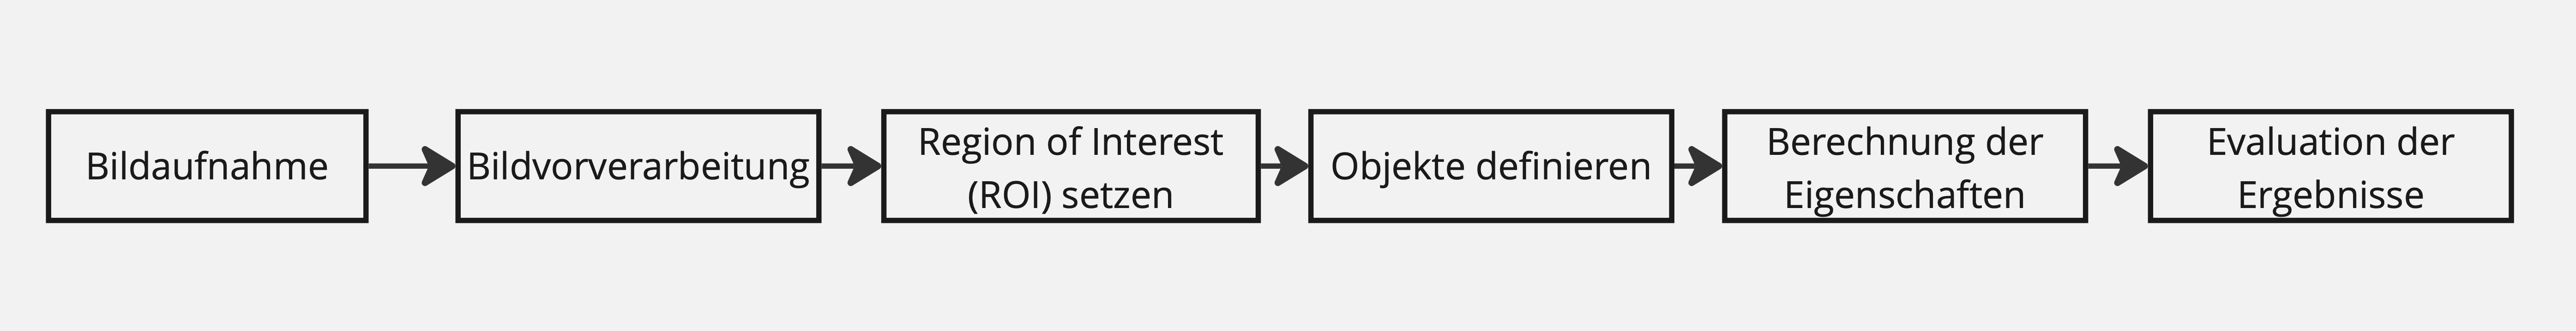
\includegraphics[width=1\linewidth]{expose/Vorgehensmodell_IBV.jpg}
    \caption{Vorgehensmodell der industriellen Sichtprüfung laut \cite[S.15]{demant_industrielle_2011}}
    \label{fig:vorgehensmodell}
\end{figure}

Dabei ist es wichtig, Bedingungen zu schaffen, unter denen eine Maschine optimal ,,sehen`` kann. Durch den Einsatz von Kameras, Beleuchtungssystemen und Bildverarbeitungsalgorithmen wird ein aussagekräftiges Bild erzeugt, um eine zuverlässige Fehlererkennung zu gewährleisten. In der Folge erfolgt eine Vorverarbeitung der Bilder unter Einsatz von Bildverbesserungsalgorithmen, um eine Optimierung der Helligkeit und des Kontrastes des Bildes zu erreichen. Die interessierenden Objekte müssen sich dabei klar von anderen Objekten und dem Hintergrund unterscheiden, um eine einfache und eindeutige Isolierung bzw. Segmentierung dieser Bereiche zu gewährleisten (\citealp[S.16]{demant_industrielle_2011};\citealp[S. 211,589]{suse_bildverarbeitung_2014}). Diese schritte erleichtern die Bildanalyse, so dass in den meisten Fällen eine \gls{od} mit einfacheren Verfahren wie das Schwellwertverfahren, Histogrammanalyse, Liniendetektion usw. möglich ist.

Im Rahmen meiner Tätigkeit wurde vorwiegend auf die firmeneigene Software Viper.NET \citealp{vipernet_about_nodate} zurückgegriffen, welche alle relevanten Schnittstellen zur Realisierung einer Bildverarbeitungssoftware bereitstellt. Für die umsetzung der Bildanalyse verwendete ich,die in der Software vorimplementierten Tools die auf basis von traditionellen Algrothmen der \gls{bv} konstuirert sind. 

Bei der behandlung eines Fallbeispiels zur Fehlererkennung wurde ersichtlich, dass bei einer starken Rauschintensität sowie einem geringen Kontrast, bei welcher eine klare Unterscheidung des Objekts vom Hintergrund nicht möglich war, keine zufriedenstellenden Resultate erzielt werden konnten. Ein Beispiel sind feine Defekte in den Musterteilen (Siehe Abbildung \ref{fig:image2}), die große Ähnlichkeiten mit den anderen Regionen des Bildes haben. Infolgedessen war keine klare, logische Abgrenzung der gesuchten Fehler zu den Musterteilen an sich möglich.Dies führte dazu, dass Bereiche des Bildes, die keinen Fehler aufwiesen, als Fehler klassifiziert wurden. Ebenso wurden Defekte nicht als solche identifiziert. Eine korrekte Detektion der Merkmale war in dem Fall mittels traditioneller Bildverarbeitungsmethoden nicht möglich.

\begin{figure}[h]

\begin{subfigure}{0.5\textwidth}
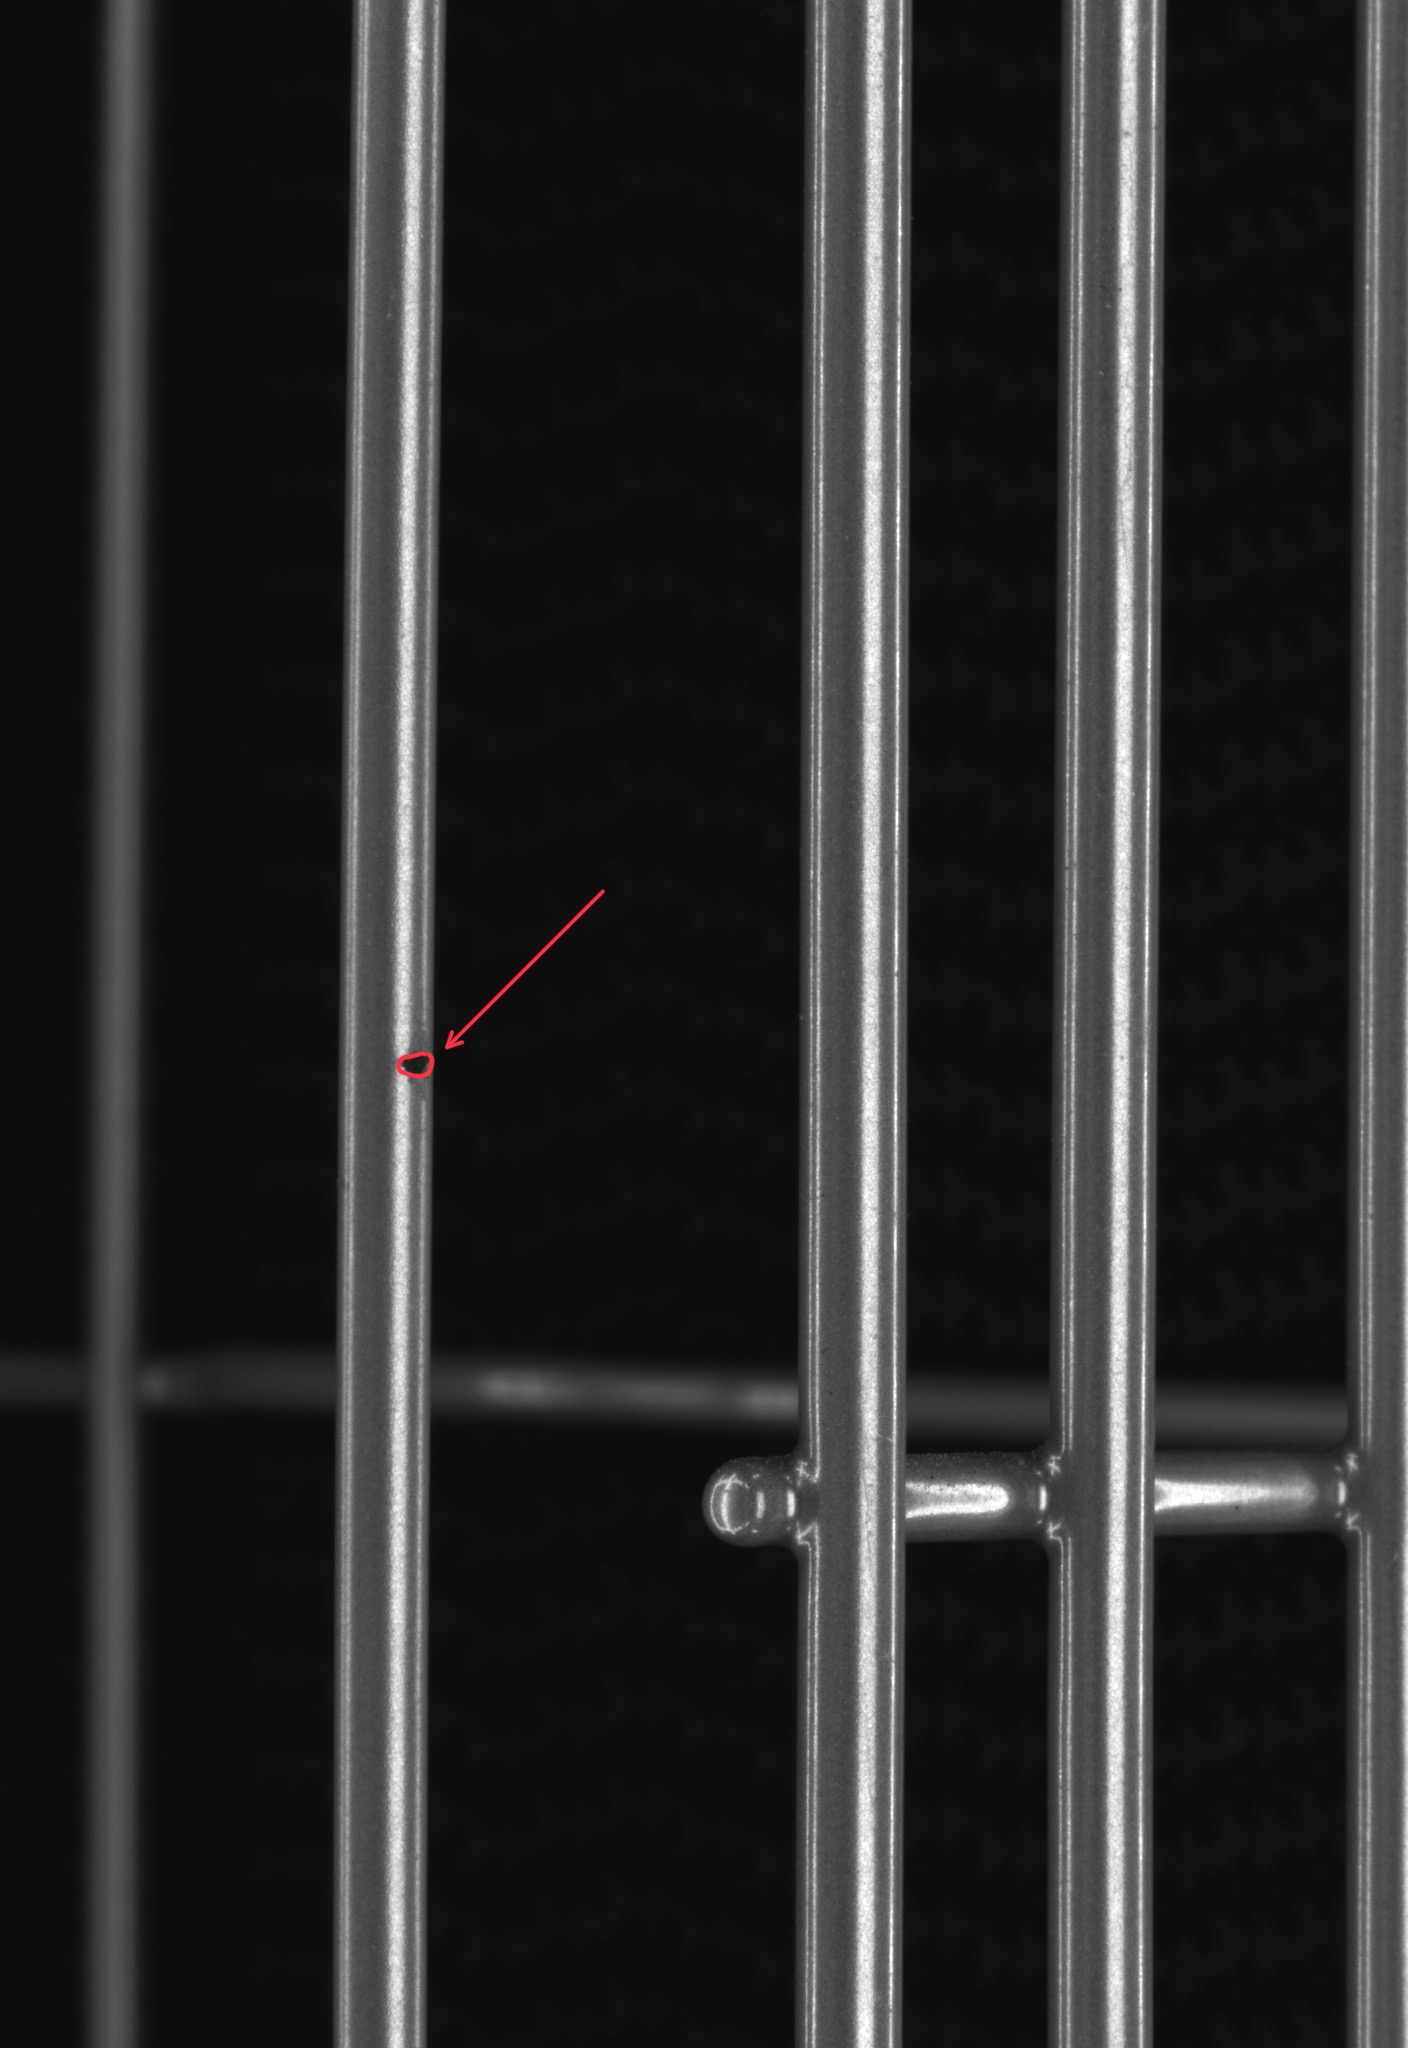
\includegraphics[width=0.9\linewidth, height=6cm]{expose/Fehler.jpg} 
\caption{Verschmutzung an einem Draht}
\label{fig:subim1}
\end{subfigure}
\begin{subfigure}{0.5\textwidth}
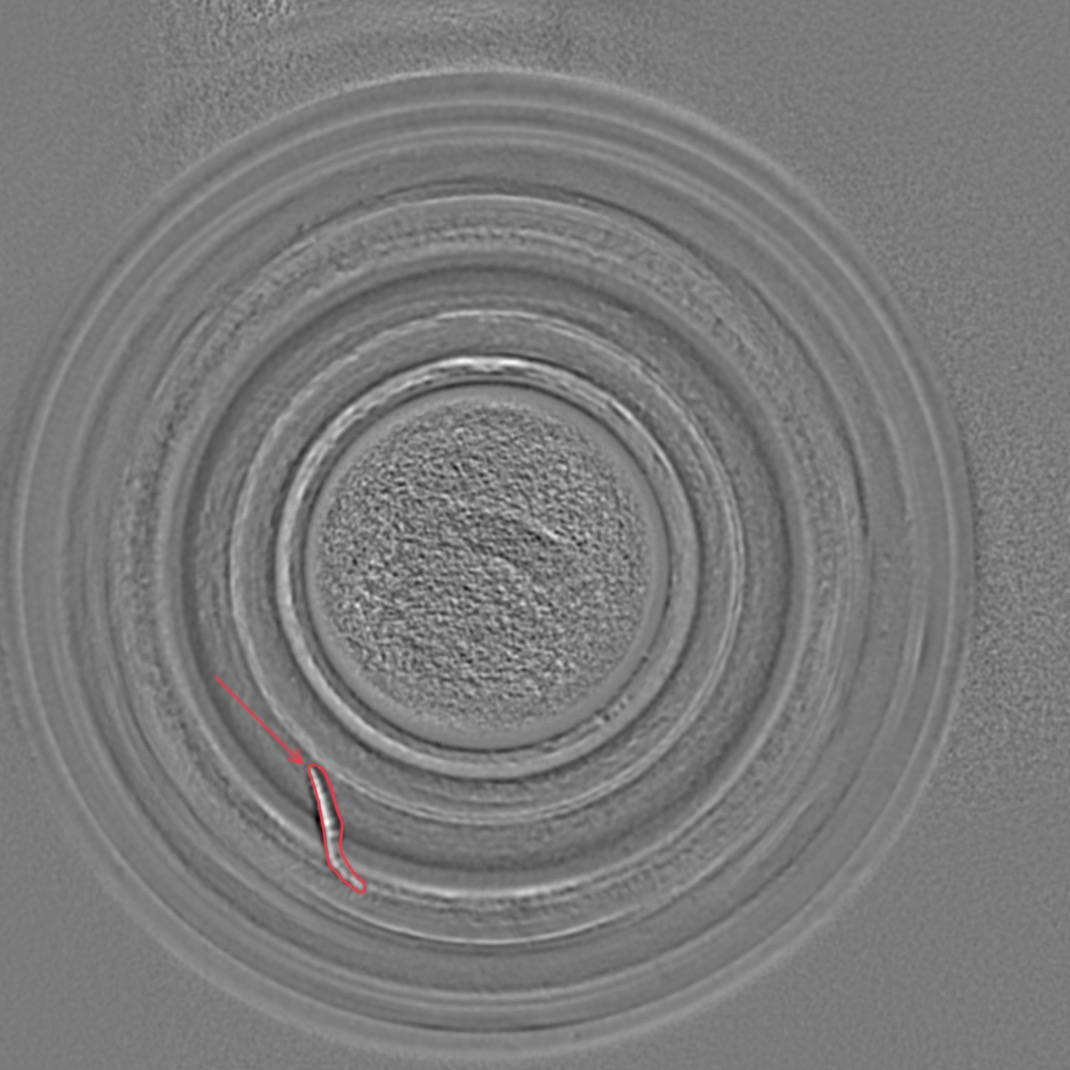
\includegraphics[width=0.9\linewidth, height=6cm]{expose/Kratzer.jpg}
\caption{Kratzer am Musterteil}
\label{fig:subim2}
\end{subfigure}

\caption{Beispiel einer Sichtprüfung aus der Praxis. Die gesuchten Merkmale wurden händisch gekennzeichnet um einen Übersicht für den Leser zu verschaffen.}

\label{fig:image2}
\end{figure}

Um die oben gennanten Herausforderungen zu lösen werden mehr fortgeschirttene Algorithmen verwendet. Dieser ansatz weckte meiner interesse, mein wissen mehr in dem Bereich der fortgeschrittenen Methoden der Objekterkennung, zu erweitern. Deep Learning algorithmen ins besondere \gls{cnn} haben sich in den letzten Jahren als effektive Methode erwiesen, um Maschinen das "Sehen" beizubringen und komplexe Muster in Bildern zu erkennen. Sie haben sich in der Bildverarbeitung etabliert, insbesondere bei Aufgaben der Bildklassifikation, Objekterkennung und Bildsegmentierung. \citealp{qi_review_2020}\citealp{manakitsa_review_2024}\citealp{kaur_systematic_2024} 

\section{Problemstellung}\label{expose_problemstellung}

Wie im \ref{expose_motivation} erwähnt, können bestimmte Eigenschaften wie spezielle Texturen, Formen, Farben oder Größen von Objekten die zuverlässige Detektion erschweren, da Fehler mit dem Hintergrund verschmelzen und somit eine präzise Analyse verhindern. Als lösung wurde eine \gls{cnn}-Basierte Objekterkennung vorgeschlagen um die Detektion von bestimmten Fehlerhaften Merkmale in Bildern zu identifizieren.

In vielen Anwendungsfällen konnte durch \gls{cnn} eine sehr hohe Genauigkeit erreicht werden. Ein Beispiel ist der Einsatz von ShuffleDefectNet, das auf einem NEU-Datensatz eine Genauigkeit von 99,75 \% erreichte. Diese Methode erfordert eine große Anzahl von fehlerfreien und fehlerhaften Beispielen in den Trainingsdaten. Das System wird mit korrekt gelabelten Daten trainiert, sodass es lernt, zwischen fehlerfreien und fehlerhaften Mustern zu unterscheiden. \cite{saberironaghi_defect_2023}

In der industriellen Sichtprüfung steht jedoch oft nur eine begrenzte Anzahl spezifischer, fehlerhafter und fehlerfreier Musterteile zur Verfügung. Da es für jeden Anwendungsfall keine öffentlich zugänglichen Datensätze gibt, entsteht ein relativ kleiner Datensatz, dessen zu detektierende Regionen manuell annotiert werden müssen.
\gls{ann} bedürfen einer überaus großen Datenmenge wenn sie mittels Supervised Learning trainiert werden. Somit kann eine gute Generalisierungsfähigkeit zu entwickeln und somit gute Ergebnisse zu liefern. \cite{lecun_deep_2015}. 

Im Rahmen meiner Forschung sind die Fortschritte im medizinischen Bereich von besonderem Interesse, da die herausforderungen und ähnlichkeiten mit meinen Datensatz übereinstimmen. Ein beispiel dafür ist das U-Net-Modell von Ronneberger et al. (2015) \cite{ronneberger_u-net_2015} von besonderer Relevanz. Dieses wurde speziell für die effiziente Segmentierung komplexer Mikroskopiebilder in der Biomedizin entwickelt und stellt somit eine wichtige Architektur in diesem Kontext dar.
Das Netzwerk wird mit sehr wenigen Bildern trainiert und zeigt dennoch eine überlegene Leistung bei Aufgaben der biomedizinischen Bildsegmentierung \cite{ronneberger_u-net_2015}. 
Es stützt sich intensiv auf Datenaugmentation, um die begrenzte Anzahl annotierter Beispiele effizient zu nutzen.
Diese Eigenschaften machen U-Net zu einem idealen Kandidaten für Anwendungen in der industriellen Qualitätskontrolle, bei denen nur eingeschränkte Trainingsdaten verfügbar sind.

In den letzten Jahren wurde die U-Net-Architektur erfolgreich in verschiedenen Bereichen der Medizin eingesetzt\cite{azad_medical_2024,siddique_u-net_2021}. Ihre Anpassungsfähigkeit und Effizienz bei der Verarbeitung komplexer Bilddaten unter schwierigen Bedingungen legen nahe, dass sie auch für die Herausforderungen in der industriellen Bildverarbeitung geeignet sein könnte.


\section{Grundlagen}

Für ein umfassendes Bildverständnis ist es nach der Erstellung eines digitalen Bildes wichtig, nicht nur das Vorhandensein bestimmter Merkmale zu erkennen, sondern auch deren genaue Position und Ausdehnung im Bild zu bestimmen. Diese Aufgabe wird als Objektdetektion definiert. Sie liefert wertvolle Informationen für das semantische Verständnis von Bildern und Videos und findet Anwendung in Bereichen wie Bildklassifikation, Verhaltensanalyse, Gesichtserkennung und autonomem Fahren \cite{zhao_object_2019}. Dennoch können Eigenschaften wie spezielle Texturen, Formen, Farben oder Größen von Objekten die zuverlässige Detektion erschweren, da Fehler mit dem Hintergrund verschmelzen und somit eine präzise Analyse verhindern.

\subsection{Deep Learning}
Convolutional Neural Networks (CNNs) haben sich hierbei als effektive Methode erwiesen, um Maschinen das "Sehen" beizubringen und komplexe Muster in Bildern zu erkennen. Sie haben sich in der Bildverarbeitung etabliert, insbesondere bei Aufgaben der Bildklassifikation, Objekterkennung und Bildsegmentierung \cite{qi_review_2020}. (Ergnzen nur hier!!!)

Ziel dieser Arbeit ist es, eine Deep-Learning-Anwendung zu entwickeln und zu evaluieren, die bestimmte gekennzeichnete Merkmale in Bildern automatisch erkennen kann. Dabei wird untersucht, wie mithilfe von CNNs und der semantischen Segmentierung trotz Herausforderungen wie begrenzter Datenmenge und Bildrauschen eine zuverlässige Erkennung möglich ist.

 In den vergangenen Jahren hat sich gezeigt, dass Deep-Learning-Modelle, insbesondere Convolutional Neural Networks (CNNs), eine neue Ära der Bildverarbeitung eingeleitet haben. Sie erzielen signifikant bessere Ergebnisse bei Aufgaben wie der Bildklassifikation, Objekterkennung und Segmentierung, was zu einer deutlichen Leistungssteigerung in verschiedenen Anwendungsbereichen geführt hat.\cite{minaee_image_2022}

Ein CNN besteht aus mehreren Schichten, von denen jede spezifische Funktionen auf die Eingabedaten anwendet. Zu den Hauptkomponenten gehören die Eingabeschicht, konvolutionale Schichten, Aktivierungsschichten, Pooling-Schichten und vollständig verbundene Schichten. Diese Architektur ermöglicht es CNNs, komplexe Merkmale aus Bildern zu extrahieren und zu interpretieren.\cite{jogin_feature_2018}